\documentclass[oneside,a4paper,12pt]{book}

\usepackage[latin1]{inputenc}
\usepackage[spanish]{babel}
\usepackage{geometry}
\usepackage{eurosym}
\usepackage{makeidx}
\usepackage{url}
\usepackage{graphicx}
\usepackage{a4wide}
\usepackage[normalsize]{subfigure}
\usepackage{named}
\usepackage{hyperref}
\usepackage{float}
\usepackage{titlesec}
\usepackage[Lenny]{fncychap}
\usepackage{babel}
\usepackage{listings}
\usepackage{fancyhdr}
\usepackage{graphicx,amscd,amsmath,amssymb,verbatim}
\usepackage{times}
\usepackage{afterpage}



% Custom colors
\usepackage{color}
\definecolor{deepblue}{rgb}{0,0,0.5}
\definecolor{deepred}{rgb}{0.6,0,0}
\definecolor{deepgreen}{rgb}{0,0.5,0}
\definecolor{gray97}{gray}{.97}
\definecolor{gray75}{gray}{.75}
\definecolor{gray45}{gray}{.45}

% Python style for highlighting
\newcommand\pythonstyle{\lstset{
language=Python,
basicstyle=\scriptsize,
otherkeywords={self},             % Add keywords here
keywordstyle=\scriptsize\color{deepblue},
emph={MyClass,__init__},          % Custom highlighting
emphstyle=\scriptsize\color{deepred},    % Custom highlighting style
stringstyle=\color{deepgreen},
frame=single,                         % Any extra options here
showstringspaces=false            % 
framerule=0pt,
aboveskip=0.5cm,
framextopmargin=3pt,
framexbottommargin=3pt,
framexleftmargin=0.4cm,
framesep=0pt,
rulesep=.4pt,
backgroundcolor=\color{gray97},
rulesepcolor=\color{black},
commentstyle=\color{gray45},
numbers=left,
numbersep=15pt,
numberstyle=\scriptsize,
numberfirstline = false,
breaklines=true,
}}


% Python style for highlighting
\newcommand\pythonstyleinline{\lstset{
language=Python,
basicstyle=\ttm,
otherkeywords={self},             % Add keywords here
keywordstyle=\color{deepblue},
emph={MyClass,__init__},          % Custom highlighting
emphstyle=\color{deepred},    % Custom highlighting style
stringstyle=\color{deepgreen},
frame=Ltb,                         % Any extra options here
showstringspaces=false            % 
framerule=0pt,
aboveskip=0.5cm,
framextopmargin=3pt,
framexbottommargin=3pt,
framexleftmargin=0.4cm,
framesep=0pt,
rulesep=.4pt,
backgroundcolor=\color{gray97},
rulesepcolor=\color{black},
commentstyle=\color{gray45},
numbers=left,
numbersep=15pt,
numberstyle=\ttm,
numberfirstline = false,
breaklines=true,
}}

% Python environment
\lstnewenvironment{python}[1][]
{
\pythonstyle
\lstset{#1}
}
{}

% Python for external files
\newcommand\pythonexternal[2][]{{
\pythonstyle
\lstinputlisting[#1]{#2}}}

% Python for inline
\newcommand\pythoninline[1]{{\pythonstyleinline\lstinline!#1!}}



%Para que no parta las palabras
\pretolerance=10000

\lhead[]{}
\chead[]{\rightmark}
\rhead[]{}
\renewcommand{\headrulewidth}{0.5pt}



% primera pagina de un capitulo
\fancypagestyle{plain}{
\fancyhead[L]{}
\fancyhead[C]{}
\fancyhead[R]{}
\fancyfoot[L]{}
\fancyfoot[C]{\thepage}
\fancyfoot[R]{}
\renewcommand{\headrulewidth}{0pt}
\renewcommand{\footrulewidth}{0pt}
}

\pagestyle{fancy}


%\DeclareGraphicsExtensions{.jpg,.pdf,.png,.ps}
\geometry{a4paper, left=3.5cm, right=2cm, top=3cm, bottom=2cm, headsep=1.5cm}

\makeindex

\begin{document}

\setlength{\emergencystretch}{2pt}
\baselineskip 1.35\baselineskip


%%%%%%%%%%%%%%%%%%%%%%%%%%%%%%%%%%%%%%%%%%%%% PORTADA Y AGRADECIMIENTOS %%%%%%%%%%%%%%%%%%%%%%%%%%%%%%%%%%%%%%%%%%%%%%%%%
\thispagestyle{empty}
\vspace{5cm}

\begin{figure}[htb]
  \centerline{\resizebox{.40\textwidth}{!}{
\includegraphics{figuras/logo_urjc.jpg}}}

\end{figure}

\begin{center}

{}
 \vspace{2cm}
  {\Large {ESCUELA T�CNICA SUPERIOR DE INGENIER�A DE TELECOMUNICACI�N}}
  \vspace{2cm}
  
  {\Large { GRADO EN INGENIER�A DE SISTEMAS AUDIOVISUALES Y MULTIMEDIA}}
  \vspace{2cm}
  
  {\Large {\bf TRABAJO FIN DE GRADO}}
  
  \vspace{2cm}

  {\Large {Seguimiento de un objeto con textura desde un drone con c�mara\\[1cm] }}

  \vspace{1cm}
  {\large {\bf Tutor}: Jos� Mar�a Ca�as Plaza \\
  {\bf Autor}: Arturo V�lez Duque}
  
  \vspace{2cm}
  
   {\large {\bf Curso acad�mico 2016-2017}}

  \vspace{2cm}
  
\end{center}




\clearpage
\thispagestyle{empty}


\afterpage{\null\newpage}
\newpage

%%%%%%%%%%%%%%%%%%%%%%%%%%%%%%%%%%%%%%%%%%%%% INDICES %%%%%%%%%%%%%%%%%%%%%%%%%%%%%%%%%%%%%%%%%%%%%%%%%%%%%%%%%%%%%%%%%%%
%\pagenumbering{roman}
%\setcounter{page}{1}
% Para que salga la bibliograf�a en el �ndice
\let\OLDthebibliography=\thebibliography
\def\thebibliography#1{\OLDthebibliography{#1}
  \addcontentsline{toc}{chapter}{\bibname}}

\frontmatter



\tableofcontents

\newpage{\ } 
\thispagestyle{empty} 
\listoffigures
\newpage{\ } 
\thispagestyle{empty} 

%\setcounter{page}{1}
%\pagenumbering{arabic}
%\listoftables

\mainmatter

%%%%%%%%%%%%%%%%%%%%%%%%%%%%%%%%%%%%%%%%%%%%% CAPITULO 1 - INTRODUCCION %%%%%%%%%%%%%%%%%%%%%%%%%%%%%%%%%%%%%%%%%%%%%%%%%
\chapter{Introducci�n}
\label{cap:Introduccion}
\setcounter{page}{1}
\hspace{1 cm}La vista es el sentido que m�s utilizamos para captar informaci�n de nuestro entorno y consiste en la habilidad de detectar la luz y de interpretarla. Tanto los humanos como los animales poseemos un sistema visual que nos permite crear un esquema de nuestro entorno y conocer detalles de los objetos que nos rodean. Gracias a estos detalles somos capaces de reconocer dichos objetos por su color, por su forma, detectar movimiento en ellos o incluso estimar aproximadamente la distancia que nos separa.\\

	Cada vez est� m�s a la orden del d�a el comportamiento aut�nomo de las m�quinas,  ya que cada d�a estas se parecen m�s al humano, gracias a que les hemos dotado de sentidos, instalando en ellas sensores con los cuales pueden percibir la realidad , como por ejemplo usando c�maras para que vean. Mediante el desarrollo de algoritmos y gracias a la capacidad de procesamiento que tienen, se pueden tratar las informaciones que reciben de sus sensores para otorgarles cierta autonom�a en funci�n de la aplicaci�n que le vayamos a dar a cada m�quina en concreto.\\

	Este trabajo de fin de grado es una aplicaci�n directa de control visual. Consiste en un sistema autom�tico que permite seguir a un objeto mediante la detecci�n de puntos de inter�s que el mismo tiene para realizar un seguimiento en un entorno en este caso virtual, pero aplicable al mundo real.\\

	Este primer cap�tulo recae en la intersecci�n entre dos campos: la rob�tica a�rea (en concreto los drones) y la visi�n artificial.
	
\section{Visi�n artificial}
\hspace{1 cm}La visi�n artificial o visi�n por computador es una disciplina cient�fica que incluye m�todos para adquirir, procesar, analizar y comprender las im�genes del mundo real con el fin de producir informaci�n num�rica o simb�lica para que puedan ser tratados por un computador.\\

	El objetivo principal que tiene esta disciplina, es que las m�quinas sean capaces de ver e interpretar el mundo como un humano lo hace observando con sus ojos y procesando la informaci�n en el cerebro. Para ello, las m�quinas encargadas de esto son dotadas de c�maras para percibir la realidad, tomando una o varias im�genes para posteriormente analizarla en su procesador. La comprensi�n de esta ``realidad'' captada por los sensores de los que dispone la maquina est� basada en el procesamiento de la imagen o im�genes gracias al an�lisis mediante algoritmos de geometr�a, estad�stica, f�sica y otras disciplinas.\\
	
	La adquisici�n de estas im�genes no siempre es perfecta, existen ruidos e interferencias de diferente naturaleza, y estas pueden provocar un mal procesamiento de la mismas dando lugar a errores. Para ello, existen diferentes t�cnicas de preprocesamiento de im�genes para que estas sean lo m�s fidedignas a la realidad.\\
	
\begin{figure} [H]
  \begin{center}
    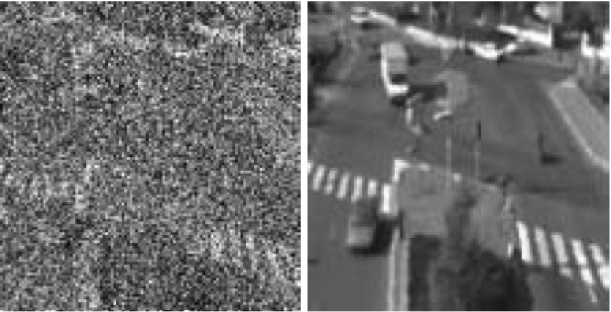
\includegraphics[width=0.5\textwidth]{figuras/ruido.jpg}
  \end{center}
  \caption{Preprocesamiento para reducci�n de ruido.}
  \label{fig:ruido}
\end{figure}

Una vez que se ha realizado el preprocesamiento de la imagen, se tiene algo muy parecido a la realidad, esta se puede utilizar con diversos fines. Dos de los m�s empleados son el aprendizaje automatizado (\textit{machine learning}) y la detecci�n de objetos.\\

	El primero utiliza t�cnicas que tienen como objetivo conseguir diferenciar autom�ticamente patrones usando algoritmos matem�ticos. Se pueden distinguir dos tipos de t�cnicas:
	
	\begin{itemize}
	\item Apredizaje supervisado: Con este aprendizaje se entrena al ordenador con patrones previamente etiquetados, de forma que el algoritmo que emplee la m�quina debe encontrar las fronteras que separan los posibles tipos de patrones.
	\item Aprendizaje no supervisado: Con este aprendizaje se entrena al ordenador con patrones que no han sido previamente clasificados y es el propio ordenador el que debe agrupar los distintos patrones en diferentes clases.
	\end{itemize} 

El segundo, la detecci�n de objetos, es la parte de la visi�n artificial que estudia c�mo detectar la presencia de objetos en una imagen sobre la base de su apariencia visual, bien sea atendiendo al tipo de objeto o a la instancia del objeto. La parte m�s importante es la extracci�n de caracter�sticas. Esta consiste en la obtenci�n de modelos matem�ticos compactos que hagan que la informaci�n de la imagen sea m�s simple con el fin de que el proceso de reconocimiento de objetos sea m�s sencillo. Las caracter�sticas que estos modelos obtienen se llaman descriptores, entre los que podemos encontrar histogramas, LBP, HOG, SIFT, SURF, ORB... Posteriormente para la b�squeda de objetos se pueden utilizar t�cnicas de aprendizaje automatizado para encontrar los clasificadores apropiados y que la detecci�n se realice correctamente.\\

\subsection{Aplicaciones}
Algunas aplicaciones que est�n teniendo mucho auge en la actualidad son el coche aut�nomo, el reconocimiento de caracteres y en medicina entre otras. Entre estas aplicaciones sin duda la que m�s destaca entre las dem�s es el coche aut�nomo debido a que ya es una realidad y podemos encontrarnos estos veh�culos en nuestras carreteras circulando entre coches no aut�nomos.\\

Los veh�culos aut�nomos perciben el entorno mediante t�cnicas complejas como l�ser, radar, lidar, sistema de posicionamiento global y visi�n computarizada. Los sistemas avanzados de control interpretan la informaci�n para identificar la ruta apropiada, as� como los obst�culos y la se�alizaci�n relevante utilizando el hardware anteriormente mencionado. Mediante las c�maras se detectan los objetos para mantener el control del veh�culo por la carretera, identificando las l�neas o los m�rgenes de estas. Tambi�n son capaces de identificar otros veh�culos y peatones prediciendo su trayectoria mediante un software desarrollado para ello. El sistema de c�mara lo complementa con un sistema de radares situados en el veh�culo con el cual son capaces de controlar con m�s precisi�n la distancia a la cual se encuentra el objeto detectado. De esta manera, el veh�culo es capaz de interpretar la realidad de una manera muy parecida a la que podr�a hacer un humano.\\

\begin{figure} [H]
  \begin{center}
    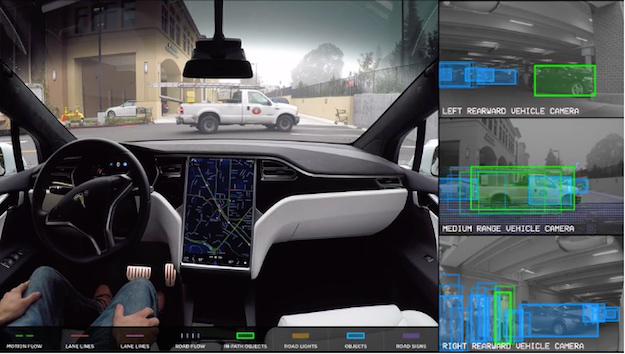
\includegraphics[width=0.5\textwidth]{figuras/autopilot.jpg}
  \end{center}
  \caption{Coche aut�nomo y los datos que procesa.}
  \label{fig:autopilot}
\end{figure}


Otra aplicaci�n es OCR, que son las siglas de \textit{Optical Character Recognition}. Como su nombre indica es un proceso dirigido a la digitalizaci�n de textos, los cuales identifican autom�ticamente, a partir de una imagen dada, s�mbolos o caracteres que pertenecen a un determinado alfabeto, para luego almacenarlos en forma de datos. As� podremos interactuar con estos mediante un programa de edici�n de texto o similar. En los �ltimos a�os la digitalizaci�n de la informaci�n (textos, im�genes, sonido, etc�tera) ha devenido un punto de inter�s para la sociedad. En el caso concreto de los textos, existen y se generan continuamente grandes cantidades de informaci�n escrita, tipogr�fica o manuscrita en todo tipo de soportes. En este contexto, poder automatizar la introducci�n de caracteres evitando la entrada por teclado implica un importante ahorro de recursos humanos y un aumento de la productividad, al mismo tiempo que se mantiene, o hasta se mejora, la calidad de muchos servicios. Tambi�n se lleva utilizando durante muchos a�os en el reconocimiento de matr�culas de veh�culos con los radares, proporcionando una cadena de caracteres que se tienen que ajustar a un modelo conocido: el formato de una matr�cula.\\

\begin{figure} [H]
  \begin{center}
    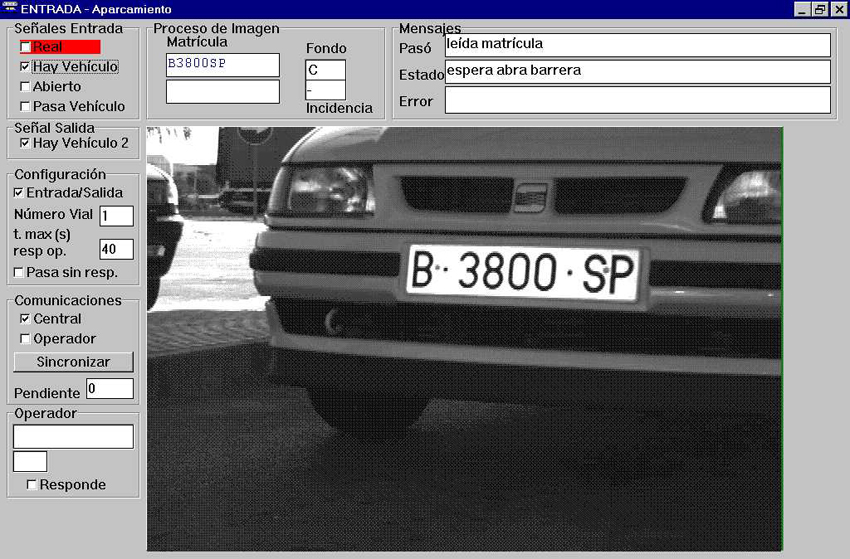
\includegraphics[width=0.5\textwidth]{figuras/matricula.jpg}
  \end{center}
  \caption{Acceso a parking mediante OCR.}
  \label{fig:matricula}
\end{figure}

El mundo de la medicina tambi�n ha aplicado la tecnolog�a de la visi�n artificial. En la medicina deportiva se est� empezando a utilizar una t�cnica de detecci�n de lesiones en atletas mediante el uso de c�maras t�rmicas. La imagen tomada por estas c�maras es procesada para localizar los puntos calientes en el cuerpo del deportista, sin�nimo de que en la zona detectada existe la posibilidad de que haya una lesi�n\footnote{http://blog.infaimon.com/2014/05/la-termografia-como-herramienta-de-diagnostico-en-medicina-deportiva/}. Tambi�n se est� desarrollando un proyecto que tiene como objetivo principal permitir a las personas sin ning�n tipo de movimiento en las extremidades superiores y que no pueden controlar los movimientos de la cabeza, controlar un rat�n del ordenador s�lo con el movimiento de los ojos mediante una c�mara y un seguimiento de los mismos \footnote{http://www.magickey.ipg.pt/}.
\\
\begin{figure}[h] % indico que voy a poner una figura y [h] indica que la posici�n relativa, tambien puedo usar t = top entre otros.
\hfill
\begin{minipage}[t]{.45\textwidth}
\begin{center}
    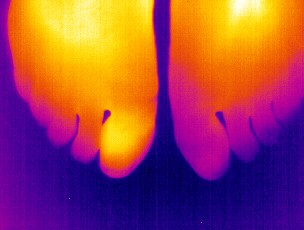
\includegraphics[width=0.8\textwidth]{figuras/termo.jpg}
  \end{center}
  \caption{Termoimagen para detecci�n de puntos calientes}
  \label{fig:termo}
\end{minipage}
\hfill
\begin{minipage}[t]{.45\textwidth}
\begin{center}
    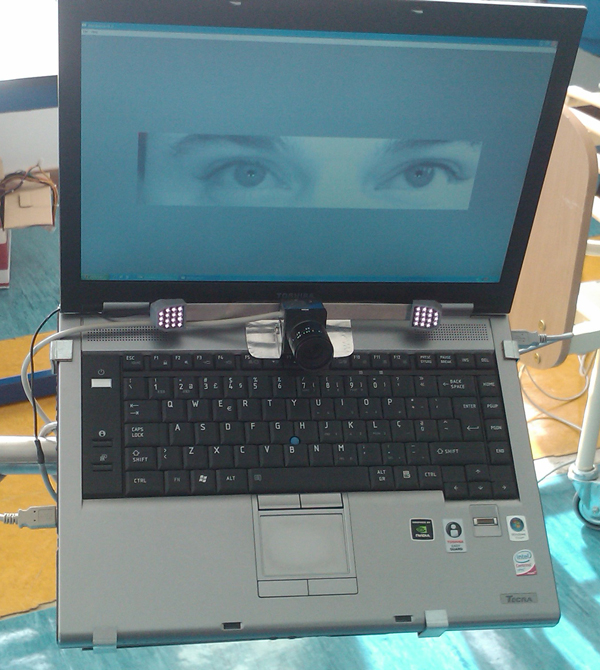
\includegraphics[width=0.8\textwidth]{figuras/ojos.jpg}
  \end{center}
  \caption{Proyecto MagicEye del Instituto Polit�cnico de Guarda}
  \label{fig:ojos}
\end{minipage}
\hfill
\end{figure}


\section{Drones (UAV)}
\hspace{1 cm}Un veh�culo a�reo no tripulado (VANT), UAV (Unmanned Aerial Vehicle) o drone es una aeronave que vuela sin tripulaci�n, concretamente se define como un veh�culo sin tripulaci�n reutilizable, capaz de mantener de manera aut�noma un nivel de vuelo controlado y sostenido siendo propulsado por uno o varios motores.\\

\begin{figure} [H]
  \begin{center}
    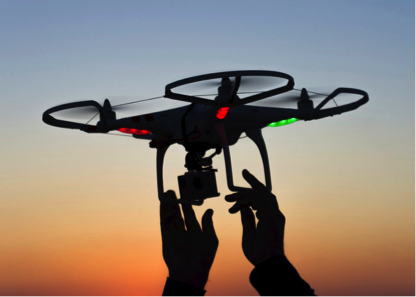
\includegraphics[width=0.5\textwidth]{figuras/dji.jpg}
  \end{center}
  \caption{Cuadric�ptero, drone con cuatro motores.}
  \label{fig:dji}
\end{figure}


Hist�ricamente, los drones se emplearon para entrenar a los soldados en el uso de ca�ones antia�reos, pero posteriormente, cuando se desarrollaron m�s era posible controlarlos remotamente gracias, en parte, a que adem�s hab�an mejorado su autonom�a. Unos de los drones m�s conocidos es el MQ-1 Predator de General Atomics, utilizado por el ej�rcito americano, primero en misiones de reconocimiento y posteriormente en misiones de ataque.\\

Actualmente el drone se ha hecho muy comercial, gracias en parte al abaratamiento de costes. Hay empresas muy importantes que comercializan estas aeronaves tales como Syma, DJI o Phantom, las cuales son tres de las m�s punteras en el �mbito de los drones. Este tipo de aparatos pueden ser equipados con c�maras entre otros tipos de sensores como GPS, IMU, bar�metro y br�julas.\\ 

\begin{figure} [H]
  \begin{center}
    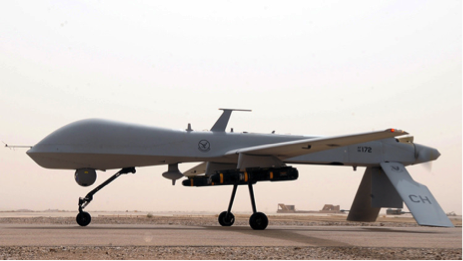
\includegraphics[width=0.5\textwidth]{figuras/predator.jpg}
  \end{center}
  \caption{Dron MQ-1 Predator equipado para ataque.}
  \label{fig:predator}
\end{figure}

Gracias a todo esto, los drones hoy en d�a son empleados en aplicaciones agr�colas, vigilancia de fronteras y terrenos, b�squedas en zonas de dif�cil acceso, topograf�a, ocio, producciones audiovisuales e inspecci�n de infraestructuras. Entre las l�neas de desarrollo en las que se esta trabajando con drones, se encuentra Amazon Prime Air \footnote{https://www.amazon.com/Amazon-Prime-Air/b?node=8037720011} e Intel Asctec Firefly \footnote{http://www.asctec.de/en/uav-uas-drones-rpas-roav/asctec-firefly/}. En primer lugar Amazon, una de las empresas l�der de compras por internet, esta desarrollando un drone con el cual podr� realizar sus entregas de una manera m�s r�pida. Este drone va equipado con c�maras con las cuales detecta las etiquetas de la persona a la cual tiene que entregar el paquete. Desde el momento en que se despacha el paquete hasta que este es recogido por el comprador, es totalmente aut�nomo. Por otro lado, el proyecto de Intel consiste en la generaci�n de un mapa 3D con unas c�maras que lleva el drone y as� controlar las distancias con los objetos, evitando colisiones.\\

\begin{figure}[h] % indico que voy a poner una figura y [h] indica que la posici�n relativa, tambien puedo usar t = top entre otros.
\hfill
\begin{minipage}[t]{.45\textwidth}
\begin{center}
    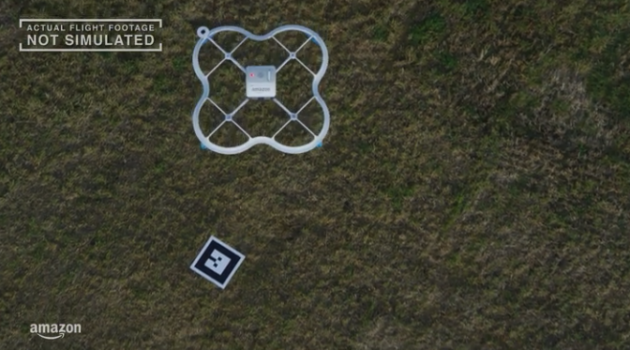
\includegraphics[width=0.8\textwidth]{figuras/amazon.jpg}
  \end{center}
  \caption{Amazon Prime Air: proceso de aterrizaje}
  \label{fig:amazon}
\end{minipage}
\hfill
\begin{minipage}[t]{.45\textwidth}
\begin{center}
    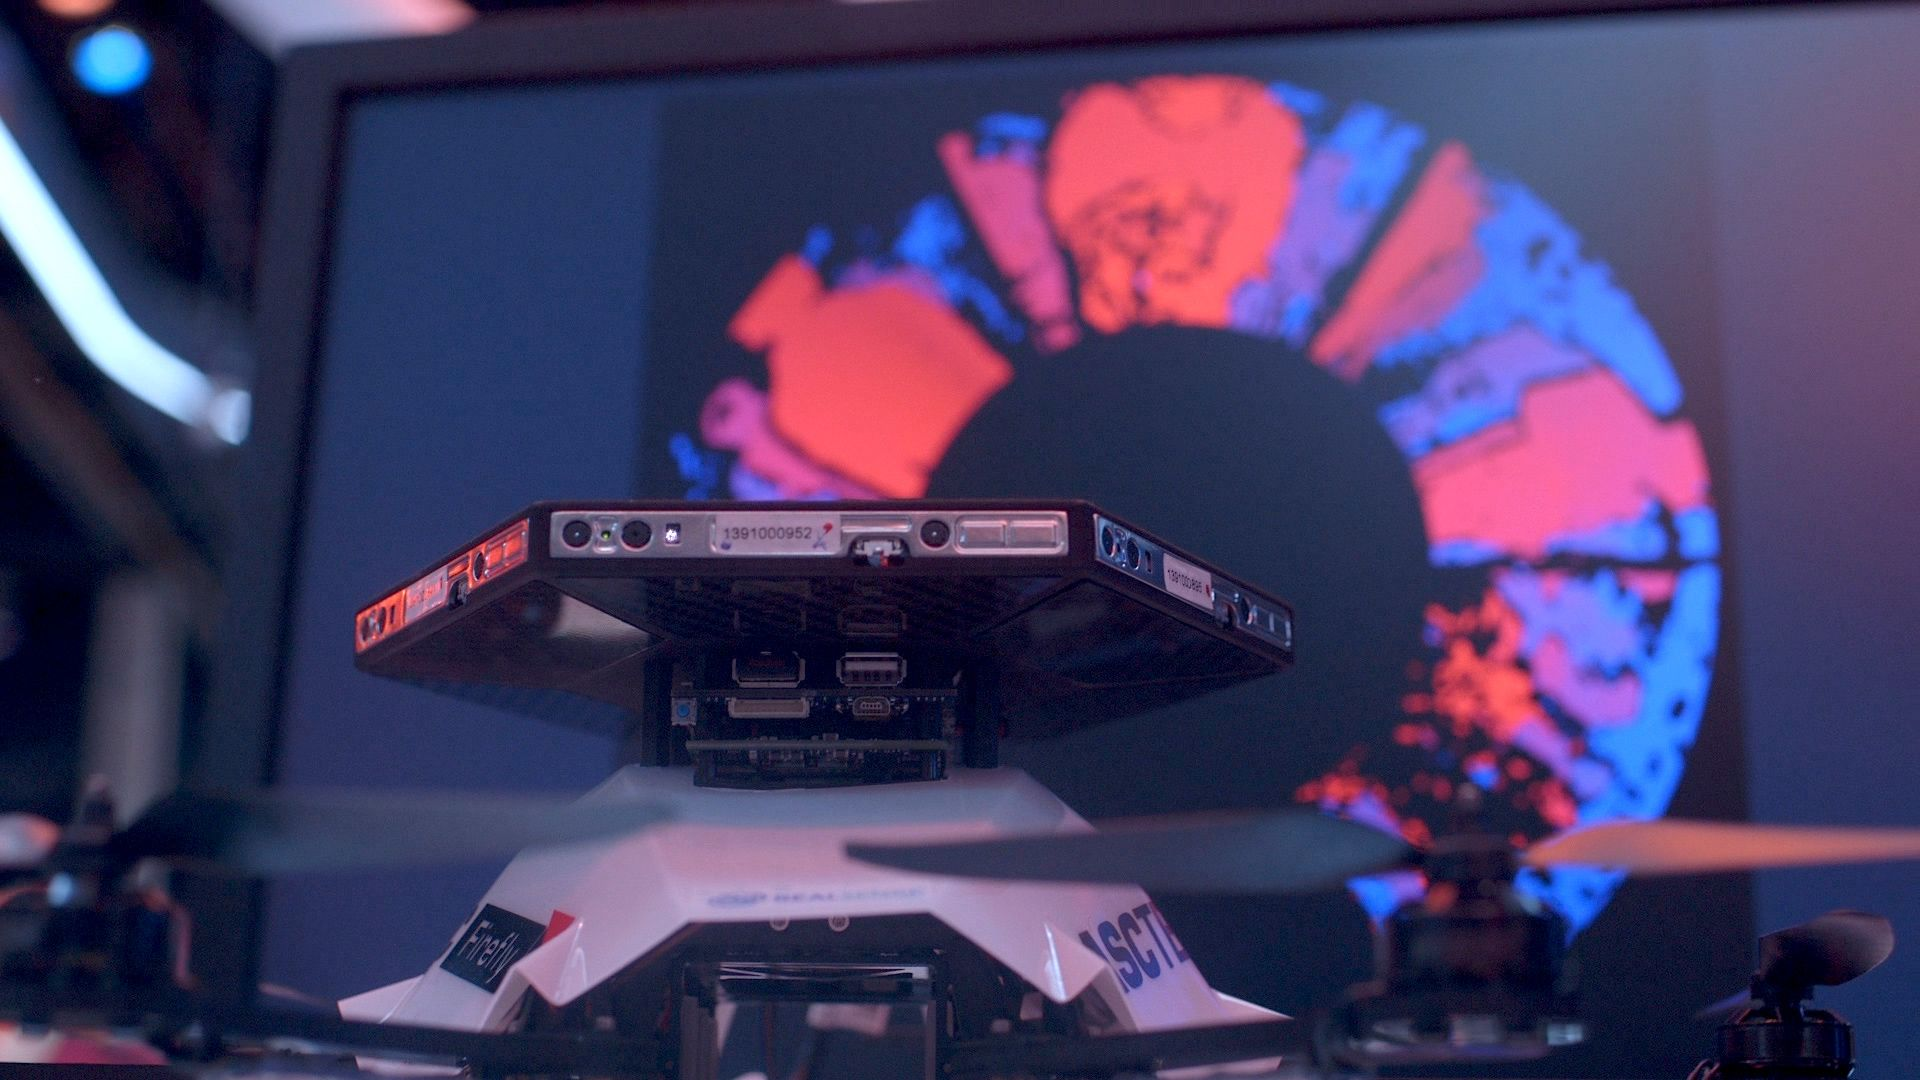
\includegraphics[width=0.8\textwidth]{figuras/asctect.jpg}
  \end{center}
  \caption{Intel Asctec Firefly: c�maras y detr�s, mapa creado}
  \label{fig:asctect}
\end{minipage}
\hfill
\end{figure}



Un drone principalmente es un robot a�reo, compuesto de hardware y software. El hardware que compone a estos robots consta de actuadores, entre los que podemos encontrar sistemas de vuelo y h�lices para otorgar la movilidad al robot, adem�s de los ya mencionados sensores que �ste puede llevar embarcados. Todo este hardware es controlado mediante un software, que puede ser de mayor o menor complejidad en funci�n del uso que se le vaya a dar al drone, pudiendo ser este controlado desde una tablet o smartphone o mediante una programaci�n de rutas. Gracias al software tambi�n se puede asumir una locomoci�n resuelta y estable gracias a los mecanismos de control implementados.\\

\subsection{Marco legal}
En conceptos legales, la nueva ley temporal que regula el uso de drones en Espa�a fue aprobada el 4 de julio de 2014. Esta nueva ley va dirigida a los drones con un peso menor de 150 kg, quedando definidas las condiciones en las que se puede emplear un drone, entre las que se encuentran: grabaci�n, vigilancia y monitorizaci�n, revisi�n de infraestructuras y obtenci�n de mapas.\\

Inicialmente los drones se categorizan seg�n su masa. Los menores de 2 kg, los que tienen entre 2 kg y 25 kg y los superiores a 25 kg. A medida que aumenta la masa, su uso est� m�s controlado. Los drones con un peso menor de 25 kg tienen una restricci�n por la que se proh�be su vuelo a altitudes superiores a 120 metros. Sea cual sea su masa, es necesario tener el carn� de piloto de drones para poder manejar estos veh�culos. Adem�s, la aeronave deber� llevar una placa identificativa con el nombre del fabricante y los datos fiscales de la empresa.\\

El carn� oficial para el manejo de drones no ser� necesario para aquellos que dispongan de un t�tulo de piloto de avi�n, ultraligero u otro espec�fico. Sin embargo, los dem�s necesitar�n pasar unos ex�menes y pruebas oficiales para obtenerlo. Es importante que la escuela en la que se realice el curso sea ATO, es decir, escuelas certificadas por AESA. Adem�s hay que tener en cuenta que hay dos cursos, uno normal y otro avanzado. El curso normal solo te habilita para volar el veh�culo mientras lo tengas a la vista y el avanzado permite todo el alcance de la aeronave.\\

En cuanto a su uso en el espacio a�reo, si se quiere utilizar un dron es necesario pedir un permiso con una antelaci�n de cinco d�as a la AESA (Agencia Estatal de Seguridad A�rea). Es muy importante recordar que est� prohibido sobrevolar n�cleos urbanos o espacios con una gran masificaci�n de gente sin el consentimiento de AESA. Por seguridad ser� necesario tener un manual de operaciones cumplimentado, adem�s de un estudio de seguridad de cada una de las operaciones que se llevar�n a cabo. Cualquier infracci�n de las normas anteriores comportar�a sanciones econ�micas de entre 3 000 y 60 000\euro.

\section{Antecedentes}
\hspace{1 cm}Es necesario situar en contexto este trabajo de fin de grado. Actualmente, hay presentados tres trabajos que guardan relaci�n con el presente. Estos son los trabajos de Aitor Mart�nez, Iv�n Rodr�guez y Alberto Mart�n Florido.\\

En los dos primeros la tem�tica principal se basa en el control de la aeronave mediante diferentes aplicaciones. En el caso de Aitor Mart�nez, su trabajo consiste no solo en el manejo de aeronaves, sino de diferentes clases de robots mediante un interfaz web. En el caso de Iv�n Rodr�guez, su trabajo consiste en el control de un drone concretamente, empleando para ello la tecnolog�a webRTC. En el �ltimo mencionado, siendo este el que m�s se asemeja al desarrollo del presente trabajo, es el proyecto llevado a cabo por Alberto Mart�n Florido. Su objetivo principal se basa en el seguimiento de objetos con unas caracter�sticas marcadas, tales como la forma y el color. Gracias a la percepci�n visual del drone y a los mecanismos de control, el drone es capaz de ejecutar su tarea y ser capaz de seguir un objeto que tenga las caracter�sticas que cumplan con los criterios.\\

Hay que destacar los trabajos desarrollados por Jorge Cano, el cual ha desarrollado un drone el cual embarca distintos dispositivos y ha desarrollado los drivers mediante los cuales ser�a posible aplicar lo desarrollado en este trabajo a un drone real, y el trabajo de Daniel Yag�e, el cual ha desarrollado lo mismo que lo anteriormente mencionado pero en en terreno virtual, pudiendo as� desarrollar el presente trabajo de fin de grado.\\

El laboratorio de rob�tica ha organizado tambi�n el campeonato de programaci�n de drones en el cual planteaban el reto de programaci�n de un drone (gato) para que busque, persiga a otro robot a�reo (rat�n) y se mantenga cerca de �l, bas�ndose en la informaci�n recibida de las c�maras que este lleva instaladas. El campeonato se desarrolla empleando un mundo virtual de Gazebo, una simulador para la creaci�n de objetos 3D que se explicar� m�s adelante.

\begin{figure} [H]
  \begin{center}
    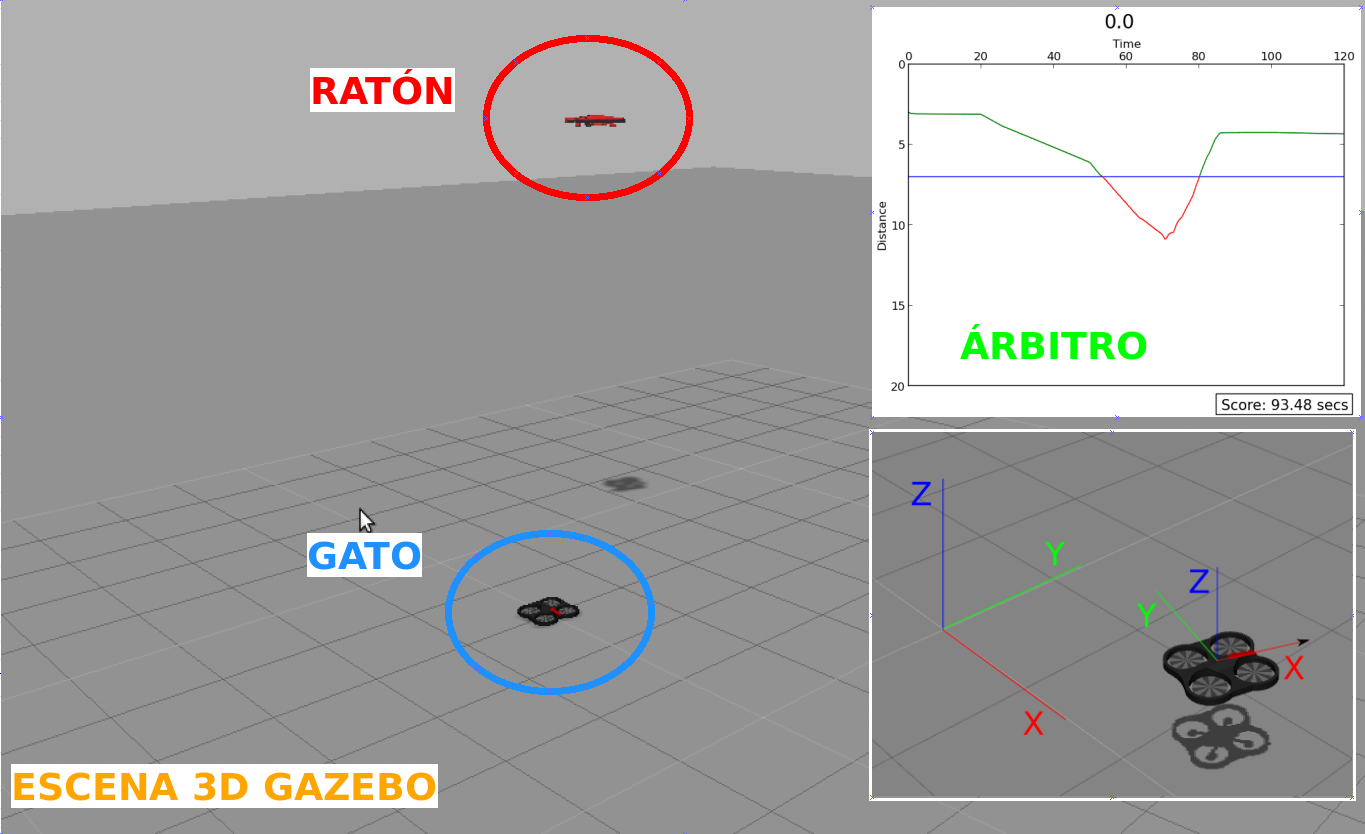
\includegraphics[width=0.5\textwidth]{figuras/gatoraton.jpg}
  \end{center}
  \caption{Campeonato de Drones de JdeRobot}
  \label{fig:gatoraton}
\end{figure}

Actualmente, en relaci�n a este tema, muchos de los problemas iniciales para la ejecuci�n de este trabajo est�n resueltos, ya que los drivers para la plataforma esta ya creado, adem�s hay aplicaciones para el control de drones mediante aplicaciones web y desde tel�fonos m�viles y ahora se esta trabajando en nuevas aplicaciones aprovechando lo que ya est� creado.\\

En el momento que se desarrollaba este trabajo de fin de grado, se estaban desarrollando paralelamente otros como por ejemplo el de Manuel Zafra, en el cual se desarrolla la navegaci�n 3D en interiores, o el de Jorge Vela, el cual desarrolla un algoritmo mediante el cual el drone es capaz de buscar y aterrizar encima de un coche, o el trabajo de Diego Jim�nez, el cual se centra menos en el procesamiento de la informaci�n tomada por los sensores y se centra en el soporte para el drone Solo Drone 3DR. \\

El presente aporta a este estado del arte una nueva forma de proceso de la informaci�n visual, siendo capaz de realizar un seguimiento de objetos m�s complejos que se asemejan m�s a la realidad, es decir, objetos con textura. En esta memoria se explica el desarrollo de esta nueva aplicaci�n empezando por los objetivos iniciales marcados, siguiendo con la infraestructura empleada y concluyendo con las pruebas y conclusiones que se han obtenido durante el desarrollo del mismo.\\







	


%%%%%%%%%%%%%%%%%%%%%%%%%%%%%%%%%%%%%%%%%%%%% CAPITULO 2 - OBJETIVOS %%%%%%%%%%%%%%%%%%%%%%%%%%%%%%%%%%%%%%%%%%%%%%%%%
\chapter{Objetivos}
\label{cap:Objetivos}
\hspace{1 cm} Una vez expuesto el contexto en el que se realiza este trabajo fin de grado, en el presente cap�tulo se detallan los objetivos concretos y requisitos de la aplicaci�n, as� como la metodolog�a y el plan de trabajo realizados. 
\section{Descripci�n del problema}
\hspace{1 cm}El objetivo global de este trabajo de fin de grado es dise�ar y programar una aplicaci�n para que un drone pueda realizar un seguimiento de objetos con textura que se mueven por una superficie. Este seguir� un objeto detectado inicialmente acorde a lo programado. El algoritmo ser� capaz de manejar un robot cudric�ptero desarrollado en un entorno simulado en 3D.\\
	
Este objetivo general se ha articulado en tres subobjetivos:
	\begin{enumerate}
    		\item{Percepci�n visual: el algoritmo ser� capaz de detectar objetos de inter�s captados mediante una c�mara y aplicando las diferentes t�cnicas de detecci�n y emparejamiento de puntos para conseguir un mecanismo de control correcto.}
   		 \item{Control del drone: se buscar� un objeto y el drone ser� capaz de seguir dicho objeto de inter�s durante toda la prueba. As� mismo, deber� localizar el objeto de inter�s en caso de p�rdida del objeto.}
    		\item{Experimentaci�n: tras el desarrollo de ambos algoritmos se pondr�n a prueba trabajando ambos a la vez y se validar� experimentalmente la soluci�n desarrollada en el drone simulado.}
	\end{enumerate}
	
\section{Requisitos}
\hspace{1cm}Los objetivos anteriormente descritos guiar�n la realizaci�n del proyecto. La soluci�n desarrollada adem�s deber�a cumplir con los siguientes requisitos:
\begin{itemize}
	\item El algoritmo tendr� que ser v�lido para su funcionamiento en JdeRobot 5.5 y Gazebo 7.4.
	\item Ser� necesario un procesamiento r�pido y vivaz del flujo de im�genes.
	\item El algoritmo tendr� que ser robusto para minimizar los errores.
	\item Los resultados deber�n ser v�lidos para diferentes tipos de objetos de inter�s.
\end{itemize} 

\section{Metodolog�a}
\hspace{1 cm} La metodolog�a seguida se ha compuesto de var�as herramientas empleadas para un avance seguro y constante en el desarrollo de los algoritmos.\\

El modo de trabajo ha seguido el desarrollo en espiral donde se iban alcanzando unos hitos para el correcto desarrollo de trabajo. Se buscaba el cierre de versiones por hito, de manera que hasta que una versi�n no estaba desarrollada y probada, no se pasaba al siguiente hito.\\

Cuando la versi�n era estable, se filmaba el resultado y se creaba una entrada en el cuaderno de bit�cora, el cual es p�blico y se puede encontrar la p�gina dedicada al trabajo de la plataforma JdeRobot\footnote{http://jderobot.org/Avelez-tfg}. Adem�s, desde el principio del desarrollo se ha utilizado un repositorio en la conocida herramienta Github.\\

Se concertaban una reuniones peri�dicas con el tutor con el cual se discut�a los problemas que se hab�a tenido durante la ejecuci�n del hito y se establec�a un nuevo hito o se prosegu�a con los mismos hasta conseguir la resoluci�n del problema y completar lo marcado.

\section{Plan de trabajo}
\hspace{1 cm}Los principales pasos seguidos durante el desarrollo del presente trabajo han sido:
	\begin{enumerate}
		\item {Aprendizaje de JdeRobot y Python: En esta fase se abordan la comprensi�n de la plataforma de JdeRobot, la instalaci�n del entorno, la interacci�n con los componentes y la compresi�n de los mismos para su posterior modificaci�n en funci�n del objetivo deseado. Tambi�n incluye el aprendizaje de la sintaxis de Python.}
		\item{Aprendizaje de ICE y Gazebo: Durante este per�odo se aprendi� la manera de funcionamiento del interfaz de comunicaciones de ICE as� mismo se empezaron a hacer las primeras pruebas con los modelos de Gazebo para comprender mejor ICE y las posibilidades que este tiene.}
		\item{Aprendizaje de OpenCV: Una vez comprendida la infraestructura a usar se pas� a aprender la biblioteca OpenCV, de una manera m�s espec�fica para el desarrollo del proyecto, aprendiendo a usar filtros de color, detecci�n de puntos y flujo �ptico, entre otras sencillas operaciones realizables por esta biblioteca.}
		\item{Desarrollo de algoritmos de detecci�n: Gracias al aprendizaje obtenido durante las fases anteriores, se ha procedido a implementar algoritmos de visi�n, como detecci�n de puntos de inter�s.}
		\item {Desarrollo de algoritmos de control: Tomando como punto de partida los datos obtenidos anteriormente, se ha desarrollado unos algoritmos capaces de enviar informaci�n precisa al drone para llevar a cabo el seguimiento del objeto, dot�ndole de autonom�a para la toma de decisiones si se encuentra con diferentes situaciones durante las pruebas.}
		\item{Validaci�n experimental: empleando el entorno simulado, se ha procedido a hacer una serie de pruebas con el fin de detectar posibles comportamientos err�neos en el drone.}
	\end{enumerate}
	
	
	
	
	

%%%%%%%%%%%%%%%%%%%%%%%%%%%%%%%%%%%%%%%%%%%%% CAPITULO 3 - INFRAESTRUCTURA %%%%%%%%%%%%%%%%%%%%%%%%%%%%%%%%%%%%%%%%%%%%%%%%%
\chapter{Infraestructura}
\label{cap:Infraestructura}
\hspace{1 cm}Para el desarrollo de este trabajo de fin de grado se ha empleado la plataforma del proyecto JdeRobot de software libre y software de terceros para la correcta ejecuci�n de los algoritmos creados.

\section{Sistema operativo virtualizado}
\hspace{1 cm} Con la mejora de las redes actuales, y la velocidad que �stas ofrecen cada vez m�s se est�n utilizando las tecnolog�as conocidas como ``\textit{cloud}'' o ``en la nube''. Este tipo de tecnolog�as consisten en una virtualizaci�n de las m�quinas en centros de datos con servidores muy potentes y con m�ltiples replicaciones de las mismas para mayor seguridad de los datos en caso de cat�strofe. Entre las empresas que ofrecen este servicio podemos encontrar Microsoft o Amazon, las cuales te permiten crear desde m�quinas muy simples a m�quinas tremendamente potentes capaces de procesar grandes cantidades de informaci�n.\\

En el caso de este proyecto, la virtualizaci�n se ha hecho localmente, en un disco duro externo. Se ha dise�ado la infraestructura de manera que la imagen pueda ser arrancada en cualquier m�quina f�sica. Para el desarrollo del trabajo de fin de grado se precisaba de un sistema operativo Ubuntu y la m�quina empleada ha sido una computadora Apple MacBook Pro con procesador Intel Core i5 de 2,4 GHz, 8GB de memoria RAM y tarjeta gr�fica Intel Iris de 1,5 GB de VRAM y todo ello con un sistema operativo Mac OS 10.12 siendo necesaria la aplicaci�n Parallels Desktop 11.0.2 para la virtualizaci�n, dotando a la maquina virtual de 4GB de memoria RAM y 256MB de VRAM, inicialmente corriendo Ubuntu 14.04 y posteriormente 16.04.\\

Durante la realizaci�n del proyecto hubo una descontinuaci�n del soporte de Parallels Desktop 11.0.2 con Ubuntu 16.04, siendo necesario la migraci�n una m�quina f�sica. Esta m�quina contaba con un procesador Intel Pentium Dual Core a 2.0 Ghz, 3GB de memoria RAM y 128MB de VRAM.\\

\section{Gazebo}
\hspace{1 cm}La simulaci�n de robots es una herramienta esencial en la caja de herramientas de un desarrollador de software para robots. Un simulador bien dise�ado permite probar r�pidamente algoritmos, dise�ar robots y realizar pruebas utilizando escenarios realistas.\\

	Gazebo\footnote{http://gazebosim.org/} es un simulador 3D de software libre que ofrece la capacidad de simular de forma precisa, realista y eficiente poblaciones de robots en entornos complejos de interior y exterior. Utiliza un  robusto motor de f�sica, gr�ficos de alta calidad y c�modas interfaces gr�ficas.\\
	
\begin{figure} [H]
  \begin{center}
    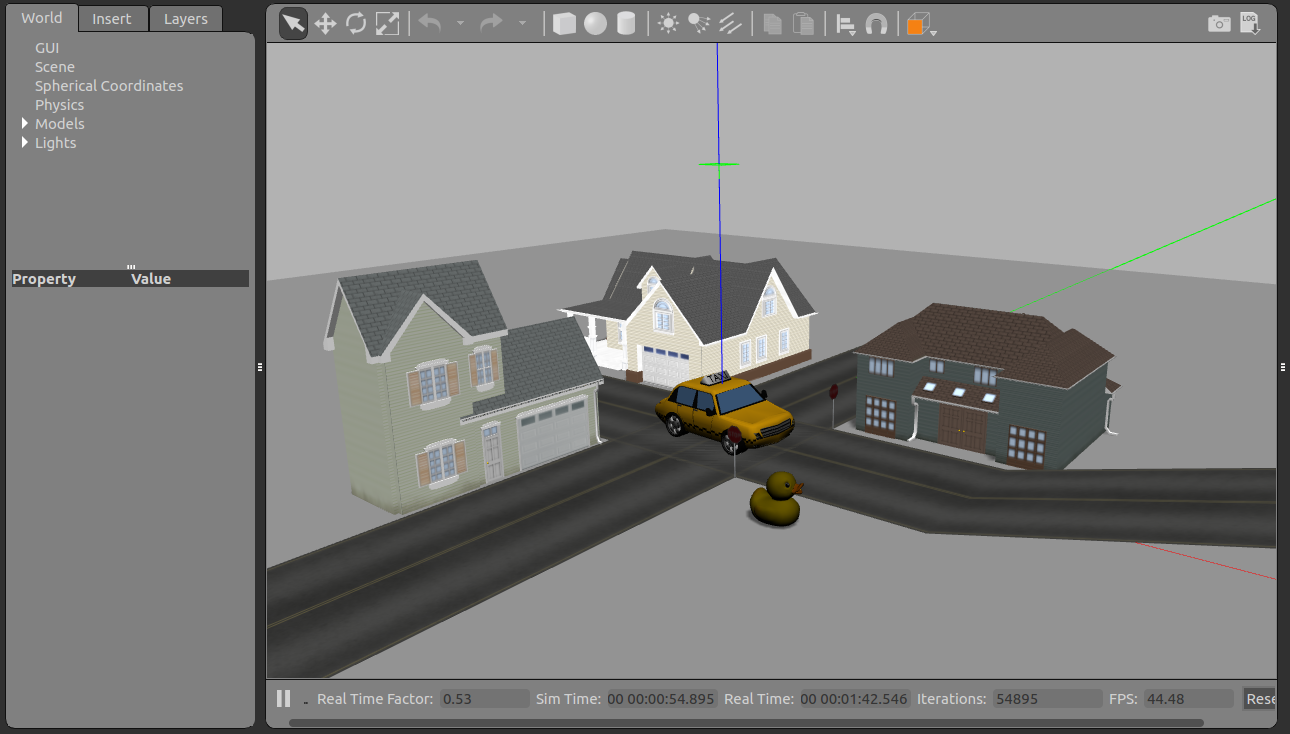
\includegraphics[width=0.7\textwidth]{figuras/robotgazebo.jpg}
  \end{center}
  \caption{Mundo simulado en Gazebo}
  \label{fig:robotgazebo}
\end{figure}

	Gracias a que hay una cantidad importante de robots y objetos dise�ados, se puede realizar todo tipo de pruebas de algoritmos de una manera muy pr�xima a la realidad pero sin la complejidad de necesitar un hardware para realizar las pruebas.\\
	
	La �ltima versi�n en la que se ha trabajado en la realizaci�n de este trabajo es la 7.4, y en esta versi�n es donde se ha realizado la experimentaci�n para validar los algoritmos desarrollados.\\
		
\subsection{ARDrone}
\hspace{1 cm}El modelo empleado para el desarrollo del proyecto ha sido el AR.Drone de la marca Parrot, o m�s bien su modelo en el entorno de simulaci�n Gazebo. Este es un drone recreativo de uso civil que fue dise�ado originalmente para  ser controlado desde un dispositivo iOs o Android, pero posteriormente Parrot liber� los applet de control bajo c�digo abierto.\\
	
\begin{figure}[h] % indico que voy a poner una figura y [h] indica que la posici�n relativa, tambien puedo usar t = top entre otros.

\hfill
\begin{minipage}[t]{.45\textwidth}
\begin{center}
    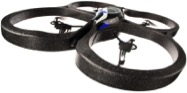
\includegraphics[width=0.8\textwidth]{figuras/ardrone.jpg}
  \end{center}
  \caption{ArDrone de Parrot}
  \label{fig:ardrone}
\end{minipage}
\hfill
\begin{minipage}[t]{.45\textwidth}
\begin{center}
    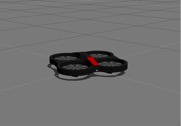
\includegraphics[width=0.8\textwidth]{figuras/ardronesim.jpg}
  \end{center}
  \caption{ArDrone simulado en Gazebo}
  \label{fig:ardronesim}
\end{minipage}
\hfill
\end{figure}

	Los algoritmos desarrollados son funcionales tanto en el drone modelado como en el drone real. Entre las especificaciones f�sicas podemos encontrar una velocidad de marcha (crucero) 5 m/s, 18 km/h y dos c�maras:
	
	\begin{itemize}
		\item{C�mara frontal con sensor CMOS de tipo gran angular de lente diagonal de 93 grados de amplitud. Resoluci�n 640x480 p�xeles (VGA). Respuesta en Frecuencia: 15 cuadros/s.}
		\item{C�mara con sensor CMOS de alta velocidad de lente diagonal. 64� de amplitud. Resoluci�n 176x144 p�xeles. Respuesta en Frecuencia: 60 cuadros/s.}
	\end{itemize}
	
	Estas caracter�sticas se han implementado en el simulador Gazebo con la generaci�n de los drivers en JdeRobot, siendo �stos los empleados en este trabajo de fin de grado. El modelo desarrollado para el simulador de entornos virtuales sigue de manera fidedigna el comportamiento, peso y manejo del modelo original pero de una manera simulada.


\section{JdeRobot}
\hspace{1 cm}JdeRobot\footnote{http://jderobot.org/} es la plataforma del laboratorio de Rob�tica de la Universidad Rey Juan Carlos. Es un entorno para el desarrollo de aplicaciones dom�ticas, rob�ticas y de visi�n artificial que se rige por los t�rminos de la licencia GNU GPL versi�n 3. JdeRobot est� orientada a componentes que funcionan de manera independiente para llevar a cabo tareas complejas. Hay componentes que sensan la realidad y env�an los datos a otros componentes que analizan los datos recibidos. La comunicaci�n entre los citados componentes se realiza mediante interfaces ICE, que abstraen de la implementaci�n de las comunicaciones.\\

\begin{figure}[h] % indico que voy a poner una figura y [h] indica que la posici�n relativa, tambien puedo usar t = top entre otros.

\hfill
\begin{minipage}[t]{.45\textwidth}
\begin{center}
    
\includegraphics[width=0.5\textwidth]{figuras/robotics.jpg}
  \end{center}
  \caption{Logo del grupo de rob�tica de la Universidad Rey Juan Carlos}
  \label{fig:robotics}
\end{minipage}
\hfill
\begin{minipage}[t]{.45\textwidth}
\begin{center}
    
\includegraphics[width=0.5\textwidth]{figuras/jderobot.jpg}
  \end{center}
  \caption{Logo de JdeRobot}
  \label{fig:jderobot}
\end{minipage}
\hfill
\end{figure}

	La arquitectura de JdeRobot est� dividida en tres partes bien diferenciadas:
\begin{enumerate}
\item{Los componentes, son las mini-aplicaciones que proveen de datos o de herramientas de an�lisis.}
\item{Las interfaces, que permiten la intercomunicaci�n entre componentes}
\item{Las bibliotecas, que facilitan el desarrollo con funcionalidades complejas.}
\end{enumerate}

	Internamente los componentes se puede dividir en dos grupos: los drivers, proporcionan los flujos de datos en bruto y las herramientas que analizan estos datos e implementan la funcionalidad final. Un ejemplo es \texttt{cameraserver} que recibe las im�genes de la c�mara y las sirve en la red a la herramienta \texttt{cameraview} que las muestra e indica los fotogramas por segundo del v�deo recibido.\\
	
	 Yendo un paso m�s existe el componente \texttt{followturtlebot}, que ha servido como base para la realizaci�n del trabajo. Este componente contiene parte de visi�n y parte de control, sirviendo de punto de partida para el desarrollo de los objetivos. Este componente incluye un interfaz gr�fico donde se puede dar �rdenes al drone, permite visualizar la c�mara y los datos de los diferentes sensores y adem�s incluye la opci�n de ver el procesamiento que se ha realizado sobre la imagen.\\
	 
	  El uso de este componente ha sido posible gracias a la utilizaci�n de \texttt{cameraserver} como servidor de im�genes. Es un driver muy �til que provee im�genes de una c�mara, de un fichero o de un flujo de datos en l�nea, lo que facilita las cosas ya que con unos sencillos cambios en el fichero de configuraci�n obtendremos las im�genes deseadas.\\
	  
	   Otro componente que cabe destacar es OpenCVDemo, que incluye funciones b�sicas de la biblioteca OpenCV, la cual se explicar� m�s adelante.\\

	Durante el desarrollo del trabajo de fin de grado se han llevado a cabo diferentes actualizaciones de la infraestructura de JdeRobot. La �ltima versi�n empleada ha sido la 5.5.\\
	

\hspace{1 cm}El lenguaje empleado en este trabajo de fin de grado es Python. Para el desarrollo de los algoritmos se han empleado fundamentalmente dos blibliotecas o paquetes que permiten a este lenguaje que realice las operaciones necesarias para el correcto funcionamiento del proyecto, adem�s de emplear una biblioteca de comunicaciones para conectar los componentes. Estas son OpenCV, Numpy y ICE. 

\section{Biblioteca de comunicaciones: ICE}
\hspace{1 cm}ICE\footnote{https://zeroc.com/products/ice} o Internet Communication Engine es un middleware orientado a objetos con soporte para diversos lenguajes de programaci�n: C++, .NET, Java, Python, ObjetiveC, Ruby y PHP. ICE provee de objetos orientados a RPC, computaci�n distribuida y servicios de publicaci�n/suscripci�n. Es desarrollado por Zeroc y tiene una licencia dual: bajo una licencia privativa y bajo GNU GPL. Se encuentra disponible en la mayor�a de los sistemas operativos actuales y tiene tambi�n una versi�n reducida para entornos m�viles.\\

\begin{figure} [H]
  \begin{center}
    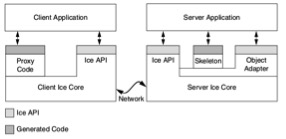
\includegraphics[width=0.5\textwidth]{figuras/ice.jpg}
  \end{center}
  \caption{Arquitectura de cliente y servidor de ICE}
  \label{fig:ice}
\end{figure}

	ICE proporciona la abstracci�n de la implementaci�n de la capa de comunicaciones a trav�s de la red. Gracias a esto es posible la comunicaci�n remota con c�maras que proveen im�genes o con otros componentes de JdeRobot. Estas interfaces se encuentran definidas en un lenguaje SLICE o Specification language for ICE que puede ser compilado en varios lenguajes de programaci�n diferentes, permitiendo el desarrollo multilenguaje de aplicaciones.\\
	
	Se ha utilizado la versi�n 3.6. La aplicaci�n desarrollada en este trabajo de fin de grado se comunica con el driver del robot simulado en Gazebo usando ICE.

\section{OpenCV}
\hspace{1 cm}OpenCV\footnote{opencv.org} es una biblioteca libre de visi�n artificial originalmente desarrollada por Intel. Desde que apareci� su primera versi�n alfa en el mes de enero de 1999, se ha utilizado en infinidad de aplicaciones. Desde sistemas de seguridad con detecci�n de movimiento, hasta aplicaciones de control de procesos donde se requiere reconocimiento de objetos. Esto se debe a que su publicaci�n se da bajo licencia BSD, que permite que sea usada libremente para prop�sitos comerciales y de investigaci�n con las condiciones en ella expresadas.\\

\begin{figure} [H]
  \begin{center}
    
\includegraphics[width=0.25\textwidth]{figuras/opencv.jpg}
  \end{center}
  \caption{Logo de OpenCV}
  \label{fig:opencv}
\end{figure}

	Open CV es multiplataforma, existiendo versiones para GNU/Linux, Mac OS X y Windows. Contiene m�s de 500 funciones que abarcan una gran gama de �reas en el proceso de visi�n.\\
	
	Esta escrita en C/C ++, la biblioteca puede aprovechar el procesamiento multi-core. Habilitando OpenCL, puede aprovechar la aceleraci�n de hardware de la plataforma empleada. OpenCV tiene m�s de 47 mil personas en la comunidad de usuarios y el n�mero estimado de descargas m�s de 9 millones. Los usos van desde el arte interactivo hasta la inspecci�n de minas, mapas en la web o la rob�tica avanzada.\\
	
	Gracias ha esta biblioteca se han podido conseguir los objetivos de percepci�n visual, ya que las funciones de las cuales dispone permiten hacer operaciones sobre las im�genes obtenidas por nuestro drone y obtener as� una serie de datos �tiles para los mecanismos de control. La versi�n utilizada para el desarrollo del trabajo de fin de grado es la 3.2.0.
	
\section{NumPy}
\hspace{1 cm}NumPy\footnote{http://www.numpy.org/} es el paquete fundamental para la computaci�n cient�fica con Python. Contiene entre otras cosas:
\begin{itemize}
	\item {Manipulaci�n de arrays de N dimensiones.}
	\item{Herramientas para integrar c�digo C / C ++ y Fortran.}
	\item{Capacidad de manipulaci�n de �lgebra lineal, transformada de Fourier y n�meros aleatorios.}
\end{itemize}

	Adem�s de sus usos cient�ficos, NumPy tambi�n puede ser utilizado como un eficiente contenedor multidimensional de datos gen�ricos y se pueden definir tipos de datos arbitrarios, esto permite a NumPy integrarse de forma transparente y r�pida con una amplia variedad de bases de datos. NumPy se licencia bajo la licencia de BSD, permitiendo la reutilizaci�n con pocas restricciones.\\
	
\begin{figure} [H]
  \begin{center}
    
\includegraphics[width=0.35\textwidth]{figuras/numpy.jpg}
  \end{center}
  \caption{Logo de Numpy}
  \label{fig:numpy}
\end{figure}

	
	
	Esta biblioteca, en su versi�n 1.12.1, ha sido utilizada para complementar a OpenCV y as� simplificar algunos de los algoritmos empleados en el trabajo de fin de grado.
	


%%%%%%%%%%%%%%%%%%%%%%%%%%%%%%%%%%%%%%%%%%%%% CAPITULO 4 - DESARROLLO %%%%%%%%%%%%%%%%%%%%%%%%%%%%%%%%%%%%%%%%%%%%%%%%%
\chapter{Desarrollo}
\label{cap:Desarrollo}

\hspace{1 cm} En este cap�tulo se describe la soluci�n dise�ada y programada para conseguir los objetivos anteriormente definidos, es decir, el desarrollo de c�mo gracias a la c�mara embarcada en el drone, en este caso, simulado, es capaz de hacer un procesamiento de la imagen y un control sobre los plugins de Gazebo para realizar la funci�n que se ha planteado.\\

El desarrollo ha consistido en 3 partes marcadas:

\begin{enumerate}
\item{Dise�o}
\item{Percepci�n visual}
\item{Algoritmos de control}
\end{enumerate}

\section{Dise�o}
\hspace{1 cm}El dise�o del componente desarrollado es muy sencillo. Por un lado se recibe las im�genes desde la c�mara del drone y se obtiene una salida en modo de movimiento del drone.\\

 \begin{figure} [H]
  \begin{center}
    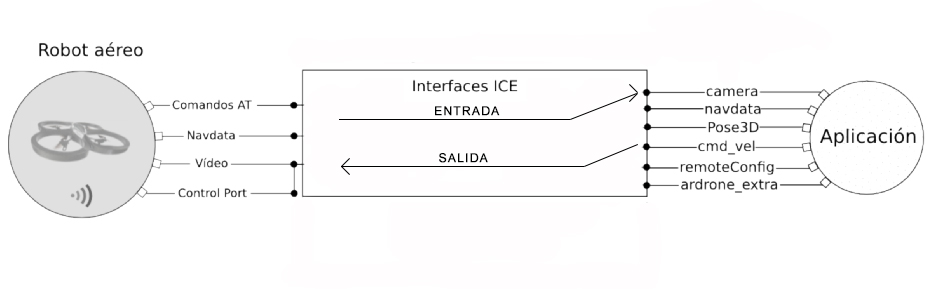
\includegraphics[width=0.5\textwidth]{figuras/esquebb.jpg}
  \end{center}
  \caption{Esquema b�sico del dise�o del componente}
  \label{fig:esquebb}
\end{figure}

Por lo tanto bas�ndonos en este esquema el drone va a tener que ser capaz de tomar imagenes, tratarlas aplicando ciertos algoritmos y con esa informaci�n utilizar algoritmos y funciones para poder tener la respuesta apropiada. Aqu� es donde se subdivide el problema en dos, parte perceptiva y parte de control:\\

\begin{figure} [H]
  \begin{center}
    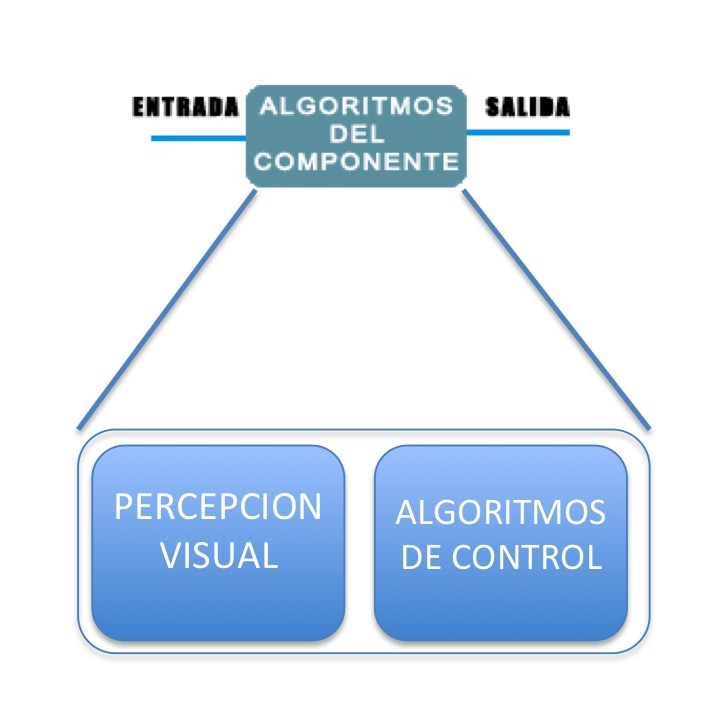
\includegraphics[width=0.5\textwidth]{figuras/esquemafull.jpg}
  \end{center}
  \caption{Esquema ampliado del componente}
  \label{fig:filter}
\end{figure}

\section{Percepci�n visual}
\hspace{1 cm} Esta parte es la primera con la que se encuentra el componente. Para obtener la entrada, el componente se conecta al interfaz de comunicaciones ICE mediante la funci�n \textbf{self.camera.getImage()}, esta funci�n se encarga de obtener las im�genes que el interfaz ofrece y este a su vez las puede obtener de diferentes fuentes, en este caso, la obtiene de la c�mara del drone simulado de Gazebo.\\

Una vez se obtiene la imagen correctamente el componente busca en la imagen el objeto de inter�s. Para ello tiene un area de b�squeda en la misma y se mantiene en ese estado hasta que el objeto aparece en la imagen.

\begin{python}[
    basicstyle=\scriptsize, %or \small or \footnotesize etc.
]
def setROI():
	global refPt, size
			
	refImg = self.camera.getImage()
	size = refImg.shape
	schSize = ((size[1]-10),(size[0]-10))
	refPt = [(10, 10), schSize]
	
\end{python}

Cuando el objeto esta en la imagen es cuando se inician los algoritmos de b�squeda de puntos. El primero con el que se encuentra es \textbf{cv2.goodFeaturesToTrack()}. Esta funci�n de OpenCV encuentra las N esquinas m�s fuertes en la imagen por el m�todo Shi-Tomasi. Este m�todo parte de la ecuaci�n $R = min(\lambda_1 , \lambda_2 )$, donde si $R$ esta por encima de un umbral, se considera como una esquina. Como de costumbre, la imagen debe ser una imagen en escala de grises. En la funci�n se especifica el n�mero de esquinas a buscar, el nivel de calidad, que es un valor entre 0-1 e indica la calidad m�nima de la esquina debajo de la cual todos son rechazados y por �ltimo proveemos la distancia euclidiana m�nima entre las esquinas detectadas. Tambi�n, a modo de hacer m�s eficiente el c�digo, elimina los puntos que est�n fuera del objeto.

\begin{python}[
    basicstyle=\scriptsize, %or \small or \footnotesize etc.
]

src = image.copy()
			
src = cv2.medianBlur(src, 3)
src_gray = cv2.cvtColor(src, cv2.COLOR_BGR2GRAY)
				
p0 = cv2.goodFeaturesToTrack(src_gray, 100, 0.01, 10, None, None, 7)
			
index = 0
if p0 != None:
	for i in (p0):
		if (i[0][0] < refPt[0][0]) or (i[0][0] > refPt[1][0]) or (i[0][1] < refPt[0][1]) or (i[0][1] > refPt[1][1]):
			p0 = np.delete(p0, index, axis=0)
		else:
			index = index + 1
\end{python}

Entonces, una vez calculados los puntos en el fotograma N, pasa a calcular la posici�n de los mismos en el fotograma N+1. Partiendo de la suposici�n de que todos los p�xeles vecinos tendr�n movimiento similar, se utiliza el metodo de Lucas-Kanade que toma un parche 3x3 alrededor del punto, as� que todos los 9 puntos tienen el mismo movimiento. Podemos encontrar $(f_x , f_y , f_t)$ para estos 9 puntos. As� que ahora nuestro problema se convierte en la soluci�n de 9 ecuaciones.\\ 

OpenCV proporciona todo esto en una sola funci�n, \textbf{cv2.calcOpticalFlowPyrLK()} que realiza el seguimiento de algunos puntos en un v�deo. La funci�n recibe el fotograma anterior, los puntos anteriores y el fotograma siguiente. Devuelve los puntos siguientes junto con algunos valores de estado que tiene un valor de 1 si se encuentra el siguiente punto, de lo contrario cero. Del mismo modo, la imagen tiene que ser en escala de grises.

\begin{python}[
    basicstyle=\scriptsize, %or \small or \footnotesize etc.
]

src2 = self.camera.getImage()
				
src2 = cv2.medianBlur(src2, 3)
src2_gray = cv2.cvtColor(src2, cv2.COLOR_BGR2GRAY)

p1, st, err = cv2.calcOpticalFlowPyrLK(src_gray, src2_gray, p0, None, None, None, 30, 30), 2, (cv2.TERM_CRITERIA_EPS | cv2.TERM_CRITERIA_COUNT, 10, 0.03))
\end{python}
 
Pero esto no es suficiente para asegurar que los puntos obtenidos son los v�lidos porque si estos llevan el esta 0 asignado no tienen punto emparejado. Por ello es necesario hacer una comprobaci�n de ese estado para ver cuales puntos est�n emparejados y cuales no. Esto lo podemos conseguir generando un array donde se van a ir almacenando todos aquellos puntos en los que su estado es 1, es decir, aquellos que estan emparejados.\\

Con los puntos v�lidos, es el momento de definir cuales son los m�s externos del objeto, lo que ayuda a definir din�micamente la regi�n de inter�s dentro de la cual va a estar el objeto.
\begin{python}[
    basicstyle=\scriptsize, %or \small or \footnotesize etc.
]
good_p1 = p1[st==1]					

maxAll = np.amax(good_p1, axis = 0)
minAll = np.amin(good_p1, axis = 0)

maxX = maxAll[0]
maxY = maxAll[1]
minX = minAll[0]
minY = minAll[1]
\end{python}

Teniendo la regi�n de inter�s donde esta contenido el objeto, la cual es rectangular, se obtiene el centro de la misma calculando el punto medio de la diagonal que une dos vertices opuestos.
\begin{python}[
    basicstyle=\scriptsize, %or \small or \footnotesize etc.
]
def squareCenter(xmax, xmin, ymax, ymin):
	global center
	center[0] = ((xmax + xmin)/2)
	center[1] = ((ymax + ymin)/2)
\end{python}

Con todo esto el componente es capaz de obtener la posici�n del objeto dentro del plano de la imagen y poder hacer un seguimiento del mismo durante todo el flujo de fotogramas de manera iterativa.\\

En ocasiones el objeto desaparecer� de la imagen, bien porque sale del plano o bien porque se hace m�s peque�o. En tal caso, los puntos soporte no podr�n ser calculados y por tanto no habr� puntos buenos  para poder realizar el seguimiento dentro de la imagen, por lo que la percepci�n del componente se reiniciar� al modo de b�squeda hasta que el objeto vuelva a aparecer en la imagen.\\

En las versiones iniciales del trabajo de fin de grado se realizaron utilizando im�genes con unas caracter�sticas muy marcadas, como por ejemplo colores fuertes para poder emplear filtros de color. Aqui la percepci�n tiene unas ligeras modificaciones.\\

En este caso la percepci�n se basa en colores y para saber si un objeto es de inter�s o no, emplea un filtro de color del cual resulta una imagen en blanco y negro donde, si el objeto tiene ese color, aparece en blanco.\\

\begin{python}[
    basicstyle=\scriptsize, %or \small or \footnotesize etc.
]
hsv = cv2.cvtColor(input_image, cv2.COLOR_BGR2HSV)

lower = np.array([50,140,50])
upper = np.array([120,255,255])

mask = cv2.inRange(hsv, lower, upper)
\end{python}

Con esta imagen binaria,e utilizan una serie de funciones que el propio OpenCV ofrece para obtener la regi�n de inter�s y el centro del mismo utilizando los momentos:

\begin{python}[
    basicstyle=\scriptsize, %or \small or \footnotesize etc.
]
contours, hierarchy = cv2.findContours(mask,cv2.RETR_TREE,cv2.CHAIN_APPROX_SIMPLE)
cnt = contours[0]
M = cv2.moments(cnt)
centroid_x = int(M['m10']/M['m00'])
centroid_y = int(M['m01']/M['m00'])
\end{python}


\section{Algoritmos de control}
\hspace{1 cm} La otra parte del componente es la encargada de controlar el drone. Para que esto sea posible, el componente hace uso de la funci�n \textbf{self.cmdvel.sendCMDVel()}, la cual conecta con el interfaz de comunicaciones ICE, que es el encargado de mandar la informaci�n que la funci�n toma de las velocidades en los ejes X, Y y Z, grado de gui�ada e inclinaci�n y la velocidad de giro entorno al eje vertical, al drone.\\

Los algoritmos de control se pueden dividir en dos:
\begin{enumerate}
\item{Algoritmos de busqueda}
\item{Algoritmos de seguimiento}
\end{enumerate}

Dentro de los algoritmos de busqueda, se desarrollaron dos, el primero se basaba en elevarse hasta encontrar el objeto, pero este no era muy util en algunas condiciones puesto que su referencia de altura se obten�a a partir del area de objetos simples. El otro m�todo empleaba un m�todo de busqueda en espiral, abriendo y cerrando la misma. Los cambios de direcci�n del drone van dirigidos por tiempo, es decir, durante 1 segundo se mueve en X, durante 2 segundos se mueve en Y, durante 3 segundos en -X, durante 4 segundos en -Y, durante 5 segundos de nuevo en X y as� sucesivamente hasta un tiempo definido experimentalmente en funci�n del tama�o del escenario.\\

Para el tiempo se tiene en cuenta el intervalo de tiempo empleado para una orden y el anterior para poder hacer esa funci�n de abrir y cerrar la espiral:
\begin{python}[
    basicstyle=\scriptsize, %or \small or \footnotesize etc.
]
def changeTime():
	global sec, secless
	if sec > secless and sec <20:
		secless = sec
		sec = sec + 1
	elif sec < secless + 2 and sec > 2:
		secless = sec
		sec = sec 
	else:
		sec = 1
		secless = 0
\end{python}

El cambio de direcci�n se hace tomando la velocidad con la que estaba movi�ndose el drone en el intervalo anterior:
\begin{python}[
    basicstyle=\scriptsize, %or \small or \footnotesize etc.
]
def changeDirection():
	global velX, velY
			
	if velX != 0.0 and velY == 0.0:
		velY = -velX
		velX = 0.0
	elif velX == 0.0 and velY != 0.0:
		velX = velY
		velY = 0.0 
\end{python}

Todo ello gobernado por la funci�n que gestiona el paso del tiempo y lanza la orden de cambio de direcci�n y aumenta el tiempo:
\begin{python}[
    basicstyle=\scriptsize, %or \small or \footnotesize etc.
]
def seek():
	global velX, velY, sec, secless
	self.cmdvel.sendCMDVel(velY, velX, 0,0,0,0)
	time.sleep(sec)
	changeTime()
	changeDirection()
\end{python}

%
%El segundo modo es con la selecci�n autom�tica del objeto. Aqu� el drone ejecuta un algoritmo de b�squeda que consiste en movimientos en espiral por el escenario de manera creciente y decreciente. El tama�o de esta espiral es en funci�n del tiempo hasta un n�mero de segundos definido experimentalmente dependiendo del tama�o del escenario en cuesti�n. Cuando el tiempo llega al m�ximo definido, el drone empieza a hacer la espiral de nuevo m�s peque�a hasta acabar en la posici�n inicial de la que hab�a partido. Este algoritmo de b�squeda se interrumpe en el momento que el drone encuentra el objeto como se ha explicado en la secci�n anterior.\\
%
%Una vez que el objeto esta localizado, tanto por el primer m�todo como por el segundo, el c�lculo del punto central de la regi�n de inter�s se calcula con una ecuaci�n de c�lculo de punto medio $C = (V_1 + V_2)/2$ donde $C$ es el punto central de la regi�n de inter�s y $V_1$ y $V_2$ los v�rtices de la misma.\\
%
%Con ese punto central se aplica la formula, igual que en la versi�n de im�genes b�sicas, $V= (R_c - C)/R_c$, donde $V$ es la velocidad, $R_c$ es el punto de referencia de la imagen y $C$ es el punto central de la regi�n de inter�s. Aqu� la diferencia con la versi�n de im�genes b�sicas es que el drone no se eleva para buscar el objeto, salvo que el usuario se lo haya ordenado y ser� su responsabilidad establecerle una altura a la cual el objeto se pueda seleccionar bien. Por lo tanto, una vez seleccionado bien el objeto, se env�a la velocidad calculada a la funci�n que se encarga del control del drone y este le persigue.\\
%
%Aqu� la capacidad de c�mputo adquiere importancia, debido a que el procesamiento de una imagen con textura requiere de m�s capacidad, por lo que la velocidad a la cual es capaz de encontrar y perseguir el drone al objeto va a venir limitada por la capacidad de procesamiento que tenga la m�quina que ejecute el algoritmo.\\ 
%
%Del mismo modo que en las im�genes b�sicas, si el drone pierde el objeto, ejecuta de nuevo los algoritmos de b�squeda, autom�tica en caso de que se este ejecutando la versi�n completamente aut�noma del drone, o bien abrir� de nuevo la ventana de selecci�n de objeto. La diferencia respecto a si un objeto est� perdido o no en esta versi�n, es que el objeto no se da por perdido solo cuando sale de la imagen, si no cuando el n�mero de puntos soporte cae por debajo de un umbral, que puede ser bien porque el objeto sale de la imagen y por lo tanto el n�mero de puntos soporte cae como es obvio por debajo del umbral, bien porque el drone se encuentra a una altura por alg�n motivo en la que no calcula bien los puntos de soporte o bien porque el objeto se mueve muy r�pido y la capacidad de c�mputo no es suficiente para calcular correctamente los puntos.\\


%%%%%%%%%%%%%%%%%%%%%%%%%%%%%%%%%%%%%%%%%%%%% CAPITULO 5 - EXPERIMENTOS %%%%%%%%%%%%%%%%%%%%%%%%%%%%%%%%%%%%%%%%%%%%%%%%%
\chapter{Experimentos}
\label{cap:Experimentos}
\hspace{1 cm} TBW

%%%%%%%%%%%%%%%%%%%%%%%%%%%%%%%%%%%%%%%%%%%%% CAPITULO 6 - CONCLUSIONES%%%%%%%%%%%%%%%%%%%%%%%%%%%%%%%%%%%%%%%%%%%%%%%%%
\chapter{Conclusiones y trabajos futuros}
\label{cap:Conclusiones y trabajos futuros}
\hspace{1 cm} El �mbito de la visi�n artificial esta ganando muchos adeptos en los �ltimos a�os debido al gran potencial que este tiene. Lo interesante de esta tecnolog�a es que algo tan normal para los humanos como es el ver y procesar la informaci�n recibida por nuestros ojos, para las m�quinas supone un reto. Gracias al desarrollo de este trabajo de fin de grado, se ha podido aprender paso a paso como las m�quinas son capaces mediante algoritmos de procesar una informaci�n recibida por un sensor y realizar una acci�n, as� como la capacidad de tomar decisiones.\\

El desarrollo no ha sido trivial, y esos retos a los que la m�quina se ha tenido que enfrentar, en el lado de la programaci�n, ha supuesto mucho esfuerzo de aprendizaje y muchas pruebas hasta al final conseguir la versi�n final donde el drone se comporta de la manera que se espera y tiene un comportamiento aut�nomo.\\

En los primeros compases era necesario aprender como ven las m�quinas y que son capaces de hacer con esa informaci�n. De ah� que las primeras pruebas que se hicieran fuesen con objetos simples, al igual que un beb� en sus primeros meses el cual interpreta de una manera mejor formas y colores sencillos en lugar de objetos m�s complejos, pero gracias a eso fundamenta su aprendizaje. Por lo tanto, una de las partes m�s importantes del presente trabajo de fin de grado fue el aprendizaje del procesamiento b�sico de im�genes y aplicar los datos del mismo a unos mecanismos de control.\\

Despu�s de ese aprendizaje b�sico, las formas b�sicas de los objetos pasan a ser puntos en una imagen real gracias a las caracter�sticas que tienen las texturas. Aqu� es donde este trabajo de fin de grado tiene su aportaci�n a este campo, debido a que apenas hay antecedentes de desarrollos que hayan tratado esta tem�tica, por lo tanto, se aporta algo novedoso, lo cual a supuesto un reto y que se ha logrado gracias a los conocimientos en el grado al cual se le pone fin con este trabajo.\\

Debido a este aprendizaje se han podido tratar los datos que las funciones ofrec�an, pudiendo desarrollar algoritmos acordes al objetivo sobre el que se centraba el tema del trabajo, generando una salida a unos datos de entrada, los cuales previamente ten�a que ser localizados haciendo necesario el desarrollo de unos algoritmos previos a esa persecuci�n.\\

Con todo esto, ha habido un aprendizaje muy �til y muy interesante para el desarrollo de tecnolog�as de visi�n artificial, ya no solo centradas en drones, si no en cualquier aspecto de la rob�tica que disponga de una c�mara y una capacidad de proceso que permita ejecutar este tipo de algoritmos.\\

\section{Trabajos futuros}
\hspace{1 cm} Como se ha mencionado al principio de este cap�tulo, la visi�n artificial dispone de un potencial alt�simo, y con el desarrollo de esta tecnolog�a de la manera apropiada, se puede conseguir desarrollar herramientas muy potentes y muy �tiles en casi cualquier campo.\\

Sin salirse demasiado de la tem�tica de un drone persiguiendo a un objeto con textura, podemos desarrollar a�n m�s este trabajo a�adiendo una clasificaci�n de caracter�sticas, es decir, haciendo que despu�s de que este obtenga las caracter�sticas, clasifique los objetos en funci�n de los datos que haya obtenido, para de este modo crear una base de datos con objetos predefinidos y desarrollar algoritmos de b�squeda que se encarguen de buscar objetos concretos dentro del espacio. Tambi�n cabe la posibilidad de desarrollar redes neuronales para que estos drones tomen decisiones m�s complejas y que aprendan.\\

En la parte del simulador Gazebo, se pueden desarrollar y se est�n desarrollando escenario m�s realistas, y empleando texturas dar� una sensaci�n de que esas pruebas est�n realizadas de la manera m�s pr�xima a la realidad\\

Respecto a los drones, se pueden desarrollar drivers para m�s modelos en el mercado, y actualmente JdeRobot est� trabajando en ello, consiguiendo que haya m�s variedad de drones disponibles para ejecutar los componentes que se desarrollen.\\

Dejando de lado un poco el tema sobre el que se ha fundamentado el trabajo, y teniendo en cuenta que el tema de la infraestructura ha sido explicado aqu�, un trabajo futuro es desarrollar im�genes de los componentes para que puedan ser plug and play, es decir, que tenga todo lo necesario para que el usuario pueda ejecutar los algoritmos sin que nada m�s sea necesario previamente, por ejemplo, poniendo esas im�genes en servicios cloud o haciendo despliegues mediante contenedores.\\

Por �ltimo, el que m�s abanico de posibilidades da para desarrollo al ser m�s general, es la visi�n artificial, en la cual se pueden desarrollar, por ejemplo, un reconocimiento facial y de gestos, y aplicar esta tecnolog�a no solo a drones sino tambi�n a sistemas de seguridad y control de maquinaria mediante la cual un coche podr�a ser conducido solamente con la mirada, apuntando con los ojos all� donde el conductor desea ir. Tambi�n se puede desarrollar un sistema de detecci�n de enfermedades en la piel mediante un reconocimiento de la textura que estas presenten, otorgando a los pacientes un m�todo de diagn�stico sin ni siquiera tener que asistir al m�dico. Podemos aplicar tambi�n el an�lisis de texturas en el mundo de las infrastructuras, por ejemplo, detectando en una pared si los ladrillos han sido correctamente colocados y si se encuentran en buen estado.\\

Esto son solo un ejemplo de las posibilidades de desarrollo que existen en el mundo de la visi�n artificial, de los drones y de los simuladores de entornos virtuales, pero las posibilidades de desarrollo de diferentes aplicaciones son casi infinitas.\\

%%%%%%%%%%%%%%%%%%%%%%%%%%%%%%%%%%%%%%%%%%%%%%%%%%%% BIBLIOGRAFIA %%%%%%%%%%%%%%%%%%%%%%%%%%%%%%%%%%%%%%%%%%%%%%%%%%%%%%%
\newpage{\ } 
\thispagestyle{empty} 


\printindex \nocite{*}
\appendix
\bibliographystyle{named} \bibliography{biblio-memoria}



\end{document}